% Layer-Aware Weighting Visualization - TikZ Figure
% Shows the sigmoid weighting function and layer importance distribution
% For IJCNN 2025 Paper

\documentclass[tikz,border=5pt]{standalone}
\usepackage{tikz}
\usepackage{pgfplots}
\pgfplotsset{compat=1.18}
\usetikzlibrary{shapes.geometric, arrows.meta, positioning, fit, backgrounds, calc, decorations.pathreplacing, patterns, pgfplots.fillbetween}

% Color scheme
\definecolor{primaryblue}{RGB}{41, 98, 255}
\definecolor{accentorange}{RGB}{255, 152, 0}
\definecolor{successgreen}{RGB}{52, 168, 83}
\definecolor{warningred}{RGB}{234, 67, 53}
\definecolor{neutralgray}{RGB}{95, 99, 104}
\definecolor{darktext}{RGB}{32, 33, 36}
\definecolor{earlylayer}{RGB}{239, 83, 80}
\definecolor{middlelayer}{RGB}{255, 193, 7}
\definecolor{latelayer}{RGB}{76, 175, 80}

\begin{document}
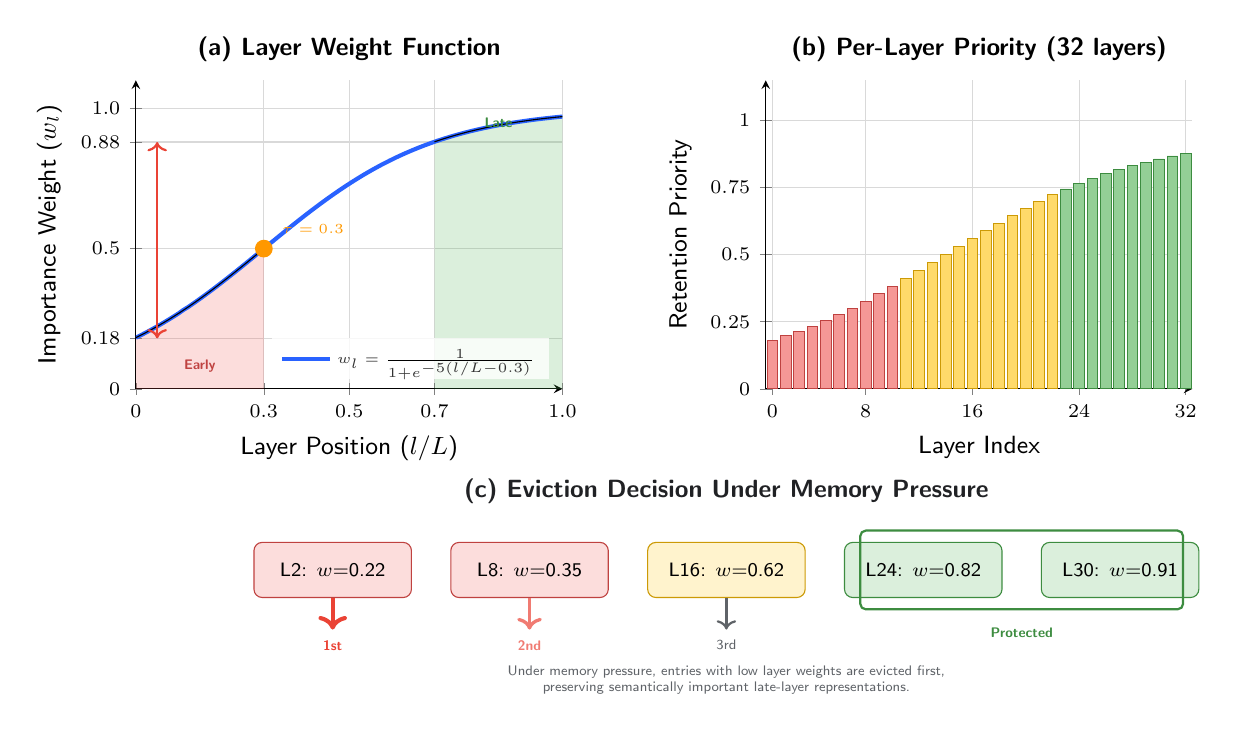
\begin{tikzpicture}

% ============================================
% Left Panel: Sigmoid Weight Function
% ============================================
\begin{axis}[
    at={(0,0)},
    width=7cm,
    height=5.5cm,
    xlabel={Layer Position ($l/L$)},
    ylabel={Importance Weight ($w_l$)},
    xmin=0, xmax=1,
    ymin=0, ymax=1.1,
    xtick={0, 0.3, 0.5, 0.7, 1.0},
    xticklabels={0, 0.3, 0.5, 0.7, 1.0},
    ytick={0, 0.18, 0.5, 0.88, 1.0},
    yticklabels={0, 0.18, 0.5, 0.88, 1.0},
    grid=major,
    grid style={gray!30},
    axis lines=left,
    xlabel style={font=\small\sffamily},
    ylabel style={font=\small\sffamily},
    tick label style={font=\scriptsize},
    title={\textbf{(a) Layer Weight Function}},
    title style={font=\small\sffamily\bfseries, yshift=-0.1cm},
    legend pos=south east,
    legend style={font=\tiny, draw=none, fill=white, fill opacity=0.8},
]

% Sigmoid curve
\addplot[
    domain=0:1,
    samples=100,
    line width=1.5pt,
    primaryblue,
    name path=sigmoid
] {1/(1 + exp(-5*(x - 0.3)))};
\addlegendentry{$w_l = \frac{1}{1+e^{-5(l/L-0.3)}}$}

% Fill regions - Early layers (0-0.3)
\addplot[
    domain=0:0.3,
    samples=50,
    name path=early
] {1/(1 + exp(-5*(x - 0.3)))};
\addplot[name path=bottom1, domain=0:0.3, draw=none] {0};
\addplot[earlylayer, fill opacity=0.2] fill between[of=early and bottom1];

% Fill regions - Late layers (0.7-1.0)
\addplot[
    domain=0.7:1,
    samples=50,
    name path=late
] {1/(1 + exp(-5*(x - 0.3)))};
\addplot[name path=bottom2, domain=0.7:1, draw=none] {0};
\addplot[latelayer, fill opacity=0.2] fill between[of=late and bottom2];

% Transition point marker
\addplot[
    only marks,
    mark=*,
    mark size=3pt,
    accentorange
] coordinates {(0.3, 0.5)};
\node[font=\tiny\sffamily, accentorange, anchor=south west] at (axis cs:0.32, 0.52) {$\tau=0.3$};

% Weight ratio annotation
\draw[<->, warningred, line width=0.8pt] (axis cs:0.05, 0.18) -- (axis cs:0.05, 0.88);
\node[font=\tiny\sffamily, warningred, anchor=east, align=right] at (axis cs:0.02, 0.53) {4.9$\times$\\ratio};

% Region labels
\node[font=\tiny\sffamily\bfseries, earlylayer!80!black] at (axis cs:0.15, 0.08) {Early};
\node[font=\tiny\sffamily\bfseries, latelayer!80!black] at (axis cs:0.85, 0.95) {Late};

\end{axis}

% ============================================
% Right Panel: Layer Importance Bars (Simplified)
% ============================================
\begin{axis}[
    at={(8cm,0)},
    width=7cm,
    height=5.5cm,
    xlabel={Layer Index},
    ylabel={Retention Priority},
    xmin=-0.5, xmax=31.5,
    ymin=0, ymax=1.15,
    xtick={0, 7, 15, 23, 31},
    xticklabels={0, 8, 16, 24, 32},
    ytick={0, 0.25, 0.5, 0.75, 1.0},
    grid=major,
    grid style={gray!30},
    axis lines=left,
    xlabel style={font=\small\sffamily},
    ylabel style={font=\small\sffamily},
    tick label style={font=\scriptsize},
    title={\textbf{(b) Per-Layer Priority (32 layers)}},
    title style={font=\small\sffamily\bfseries, yshift=-0.1cm},
]

% Early layers (red)
\addplot[
    ybar,
    bar width=0.8,
    fill=earlylayer!60,
    draw=earlylayer!80!black,
    line width=0.3pt,
] coordinates {
    (0, 0.182) (1, 0.198) (2, 0.215) (3, 0.234) (4, 0.255)
    (5, 0.277) (6, 0.301) (7, 0.327) (8, 0.354) (9, 0.382)
};

% Middle layers (yellow/orange)
\addplot[
    ybar,
    bar width=0.8,
    fill=middlelayer!60,
    draw=middlelayer!80!black,
    line width=0.3pt,
] coordinates {
    (10, 0.411) (11, 0.440) (12, 0.470) (13, 0.500) (14, 0.530)
    (15, 0.560) (16, 0.589) (17, 0.618) (18, 0.646) (19, 0.673)
    (20, 0.698) (21, 0.723)
};

% Late layers (green)
\addplot[
    ybar,
    bar width=0.8,
    fill=latelayer!60,
    draw=latelayer!80!black,
    line width=0.3pt,
] coordinates {
    (22, 0.745) (23, 0.766) (24, 0.785) (25, 0.802) (26, 0.818)
    (27, 0.832) (28, 0.845) (29, 0.857) (30, 0.868) (31, 0.878)
};

% Eviction direction arrows
\draw[->, line width=1.2pt, warningred] (axis cs:2, -0.08) -- (axis cs:10, -0.08);
\node[font=\tiny\sffamily, warningred, anchor=north] at (axis cs:6, -0.08) {Evict First};

\draw[->, line width=1.2pt, latelayer] (axis cs:29, -0.08) -- (axis cs:21, -0.08);
\node[font=\tiny\sffamily, latelayer!80!black, anchor=north] at (axis cs:25, -0.08) {Keep Longer};

% Layer type brackets
\draw[decorate, decoration={brace, amplitude=5pt, mirror}, line width=0.8pt, earlylayer!80!black]
    (axis cs:-0.5, -0.18) -- (axis cs:9.5, -0.18);
\node[font=\tiny\sffamily, earlylayer!80!black, anchor=north] at (axis cs:4.5, -0.25) {Early (0-30\%)};

\draw[decorate, decoration={brace, amplitude=5pt, mirror}, line width=0.8pt, middlelayer!80!black]
    (axis cs:10.5, -0.18) -- (axis cs:21.5, -0.18);
\node[font=\tiny\sffamily, middlelayer!80!black, anchor=north] at (axis cs:16, -0.25) {Middle};

\draw[decorate, decoration={brace, amplitude=5pt, mirror}, line width=0.8pt, latelayer!80!black]
    (axis cs:22.5, -0.18) -- (axis cs:31.5, -0.18);
\node[font=\tiny\sffamily, latelayer!80!black, anchor=north] at (axis cs:27, -0.25) {Late (70-100\%)};

\end{axis}

% ============================================
% Bottom Panel: Eviction Example
% ============================================
\node[font=\small\sffamily\bfseries, darktext] at (7.5, -1.3) {\textbf{(c) Eviction Decision Under Memory Pressure}};

% Cache entries
\node[draw=earlylayer!80!black, fill=earlylayer!20, rounded corners=3pt, minimum width=2cm, minimum height=0.7cm, font=\scriptsize\sffamily] (e1) at (2.5, -2.3) {L2: $w$=0.22};
\node[draw=earlylayer!80!black, fill=earlylayer!20, rounded corners=3pt, minimum width=2cm, minimum height=0.7cm, font=\scriptsize\sffamily] (e2) at (5, -2.3) {L8: $w$=0.35};
\node[draw=middlelayer!80!black, fill=middlelayer!20, rounded corners=3pt, minimum width=2cm, minimum height=0.7cm, font=\scriptsize\sffamily] (e3) at (7.5, -2.3) {L16: $w$=0.62};
\node[draw=latelayer!80!black, fill=latelayer!20, rounded corners=3pt, minimum width=2cm, minimum height=0.7cm, font=\scriptsize\sffamily] (e4) at (10, -2.3) {L24: $w$=0.82};
\node[draw=latelayer!80!black, fill=latelayer!20, rounded corners=3pt, minimum width=2cm, minimum height=0.7cm, font=\scriptsize\sffamily] (e5) at (12.5, -2.3) {L30: $w$=0.91};

% Eviction order
\draw[->, line width=1.5pt, warningred] (e1.south) -- ++(0, -0.4) node[below, font=\tiny\sffamily\bfseries, warningred] {1st};
\draw[->, line width=1.2pt, warningred!70] (e2.south) -- ++(0, -0.4) node[below, font=\tiny\sffamily\bfseries, warningred!70] {2nd};
\draw[->, line width=0.8pt, neutralgray] (e3.south) -- ++(0, -0.4) node[below, font=\tiny\sffamily, neutralgray] {3rd};

% Protected label
\node[font=\tiny\sffamily\bfseries, latelayer!80!black] at (11.25, -3.1) {Protected};
\draw[latelayer!80!black, line width=0.8pt, rounded corners=2pt] (9.2, -2.8) rectangle (13.3, -1.8);

% Caption
\node[font=\tiny\sffamily, neutralgray, align=center] at (7.5, -3.7) {Under memory pressure, entries with low layer weights are evicted first,\\preserving semantically important late-layer representations.};

\end{tikzpicture}
\end{document}
